\documentclass{ctexart}

\title{LSM Tree实验报告}
\author{陈天予 519021910045}
\date{\today}
\usepackage{natbib}
\usepackage{graphicx}
\usepackage{enumitem}
\usepackage{subfigure}

\begin{document}

\maketitle

\section{背景介绍}
LSM Tree(Log-structure Merge Tree)数据结构,于1996年在Patrick O’Neil 等人的一篇论文提出。其通过SS-Table的多层储存结构,利用磁盘顺序读写的高效性,实现了性能极高的写操作。LSM Tree被广泛地在各种NoSQL中使用,比如HBase,LevelDB等。

\section{挑战}
\begin{enumerate}
  \item 持久化:之前写过的程序,数据结构都在内存中,很少涉及到文件的读写。LSM Tree通过客制化结构的SSTable实现持久化,需要通过二进制的方式来读写sst文件,因不熟悉c++相关的库函数而导致的bug就不少。
  \item sst文件的debug:由于sst文件在硬盘中,debug的过程中无法实时看到其中的数据,造成许多麻烦和障碍。最终写了一个peekSSTable的小程序扫描各层sst文件并输出debug信息,解决了debug时的困难。
  \item 一个难以复现的bug:在调试过程中,有一次发现一个难以复现的bug,复盘半天发现一个现象,如果两次debug时间间隔较长,这个bug就不会出现,反之就有很高机率出现。最终发现竟然是一个函数中忘记关闭文件,使得打开了过多的文件,在操作系统还未回收完这些fd前运行程序就有可能出现这个bug。
  \item 测试脚本和测试数据的构思:这应该是第一次接触较复杂的程序性能衡量,需要自己写测试脚本,与真实环境尽量相符;并通过不同的数据集,反应程序在不同时间,不同使用角度的性能。
\end{enumerate}

\section{测试}

\subsection{测试环境和脚本说明}
AMD R7 3700x with SSD in Ubuntu 20.04 LTS\\
测试的两个脚本在delay.cpp与compaction.cpp中,使用make delay和make compaction来编译。

\subsection{性能测试}

\subsubsection{测试方法}
插入1000个随机大小在1 Byte到近2 MB的字符串(总数据量大约在1G左右),随后打乱所有keys,执行GET操作,再打乱所有keys,执行DELETE操作。重复上述方法连续测试三次,测试各方法的平均延时和吞吐。
\subsubsection{预期结果}
\begin{enumerate}
  \item 对每次测试:测试结果应该相近。
  \item 对PUT操作:随着插入数据量的增大,触发compaction的机率也越大,吞吐也越低。
  \item 对PUT操作:随着GET数据量的增大,吞吐也会越低。
  \item 对DELETE操作:由于DELETE操作相当于插入一个小字符串,所以对于不同大小的数据吞吐应该相同。但由于在del需要先判断key是否在数据库中,所以总体来说,其吞吐量趋势应与PUT类似,并稍低一些,因为其有可能触发compaction操作。
\end{enumerate}

\subsubsection{实际结果}
测试的结果如下:
\begin{verbatim}
    >>>>> Put Test <<<<<
    0...100...200...300...400...500...600...700...800...900...
    Average Delay For Different Size Data:
    0 ~ 0.25MB     : 3.94ms throughput: 254.00/s
    0.25MB ~ 0.5MB : 8.80ms throughput: 113.58/s
    0.5MB ~ 1MB    : 21.98ms throughput: 45.49/s
    1MB ~ 1.5MB    : 42.43ms throughput: 23.57/s
    1.5MB ~ 2MB    : 44.75ms throughput: 22.35/s
    
    Average Delay: 28.00ms, Average Throughput: 35.72/s
    Total Size Insert: 961MB
    
    >>>>> Get Test <<<<<
    Average Delay And Throughput For Different Size Data:
    0 ~ 0.25MB     : 98.67µs throughput: 10134.66/s
    0.25MB ~ 0.5MB : 137.13µs throughput: 7292.47/s
    0.5MB ~ 1MB    : 180.61µs throughput: 5536.77/s
    1MB ~ 1.5MB    : 238.53µs throughput: 4192.35/s
    1.5MB ~ 2MB    : 292.84µs throughput: 3414.80/s
    
    Average Delay: 203.35µs, Average Throughput: 4917.65/s
    
    >>>>> Delete Test <<<<<
    Average Delay And Throughput For Different Size Data:
    0 ~ 0.25MB     : 100.34µs throughput: 9965.85/s
    0.25MB ~ 0.5MB : 142.98µs throughput: 6993.74/s
    0.5MB ~ 1MB    : 192.80µs throughput: 5186.74/s
    1MB ~ 1.5MB    : 262.21µs throughput: 3813.78/s
    1.5MB ~ 2MB    : 327.54µs throughput: 3053.05/s
    
    Average Delay: 221.23µs, Average Throughput: 4520.18/s
    
    >>>>> Summary <<<<<
    It takes 28s to complete the test.
\end{verbatim}

\subsubsection{结果分析}
测试结果与预期相符。不足之处在于PUT操作的测试颗粒度不够,对于小数据量的测试不够完全。
\begin{figure}[h!]
  \centering
  \subfigure[GET]
  {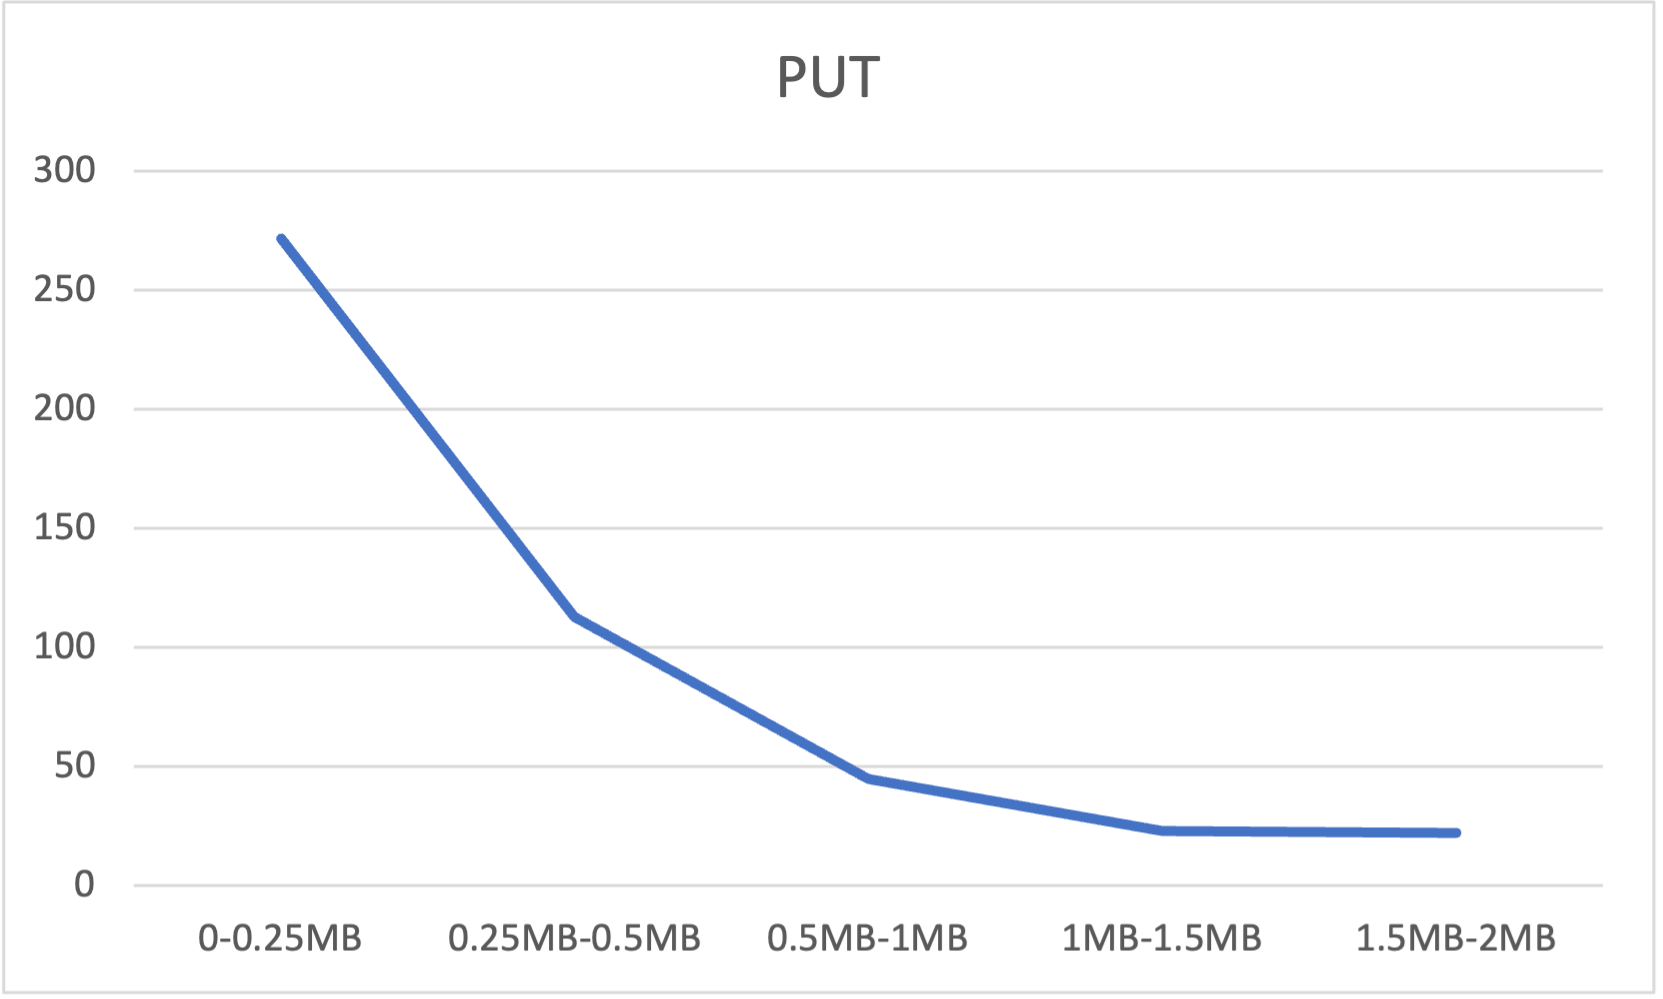
\includegraphics[width=5cm]{GET.png}}
  \subfigure[PUT \& DELETE]
  {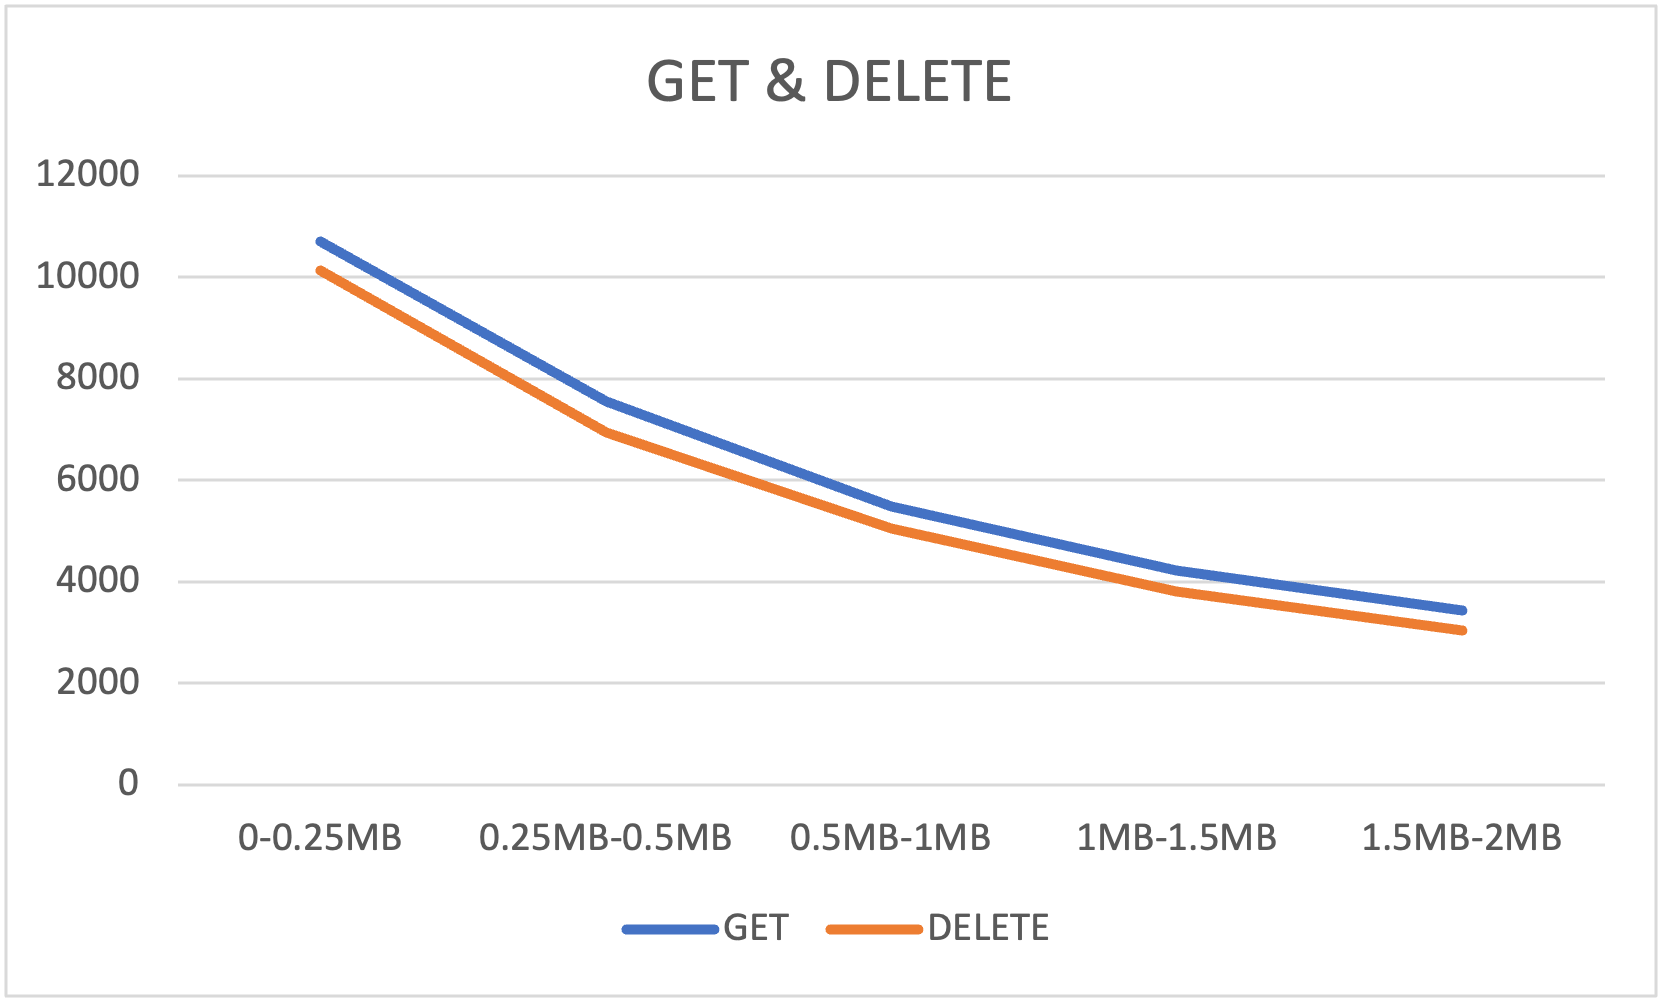
\includegraphics[width=5cm]{PUT-DELETE.png}}
  \caption{各操作对不同数据量的吞吐}
\end{figure}


\subsection{索引缓存与Bloom Filter的效果测试}

\subsubsection{测试方法}
测试脚本与性能测试相同,不同版本的代码存放在不同的git分支中,其中无缓存版本对应着naive分支,缓存索引信息的版本对应着index\_cached分支,完全版本在index\_cached\_with\_bf分支中。

\subsubsection{预期结果}
三种测试中GET操作的平均时延应有显著差距,但同种测试之间对不同数据大小的时延变化趋势应与性能测试中的相同。

\subsubsection{实际结果}
因篇幅限制,实际输出放在了cache\_test.md中,这里只放图表。
\begin{figure}[h!]
  \centering
  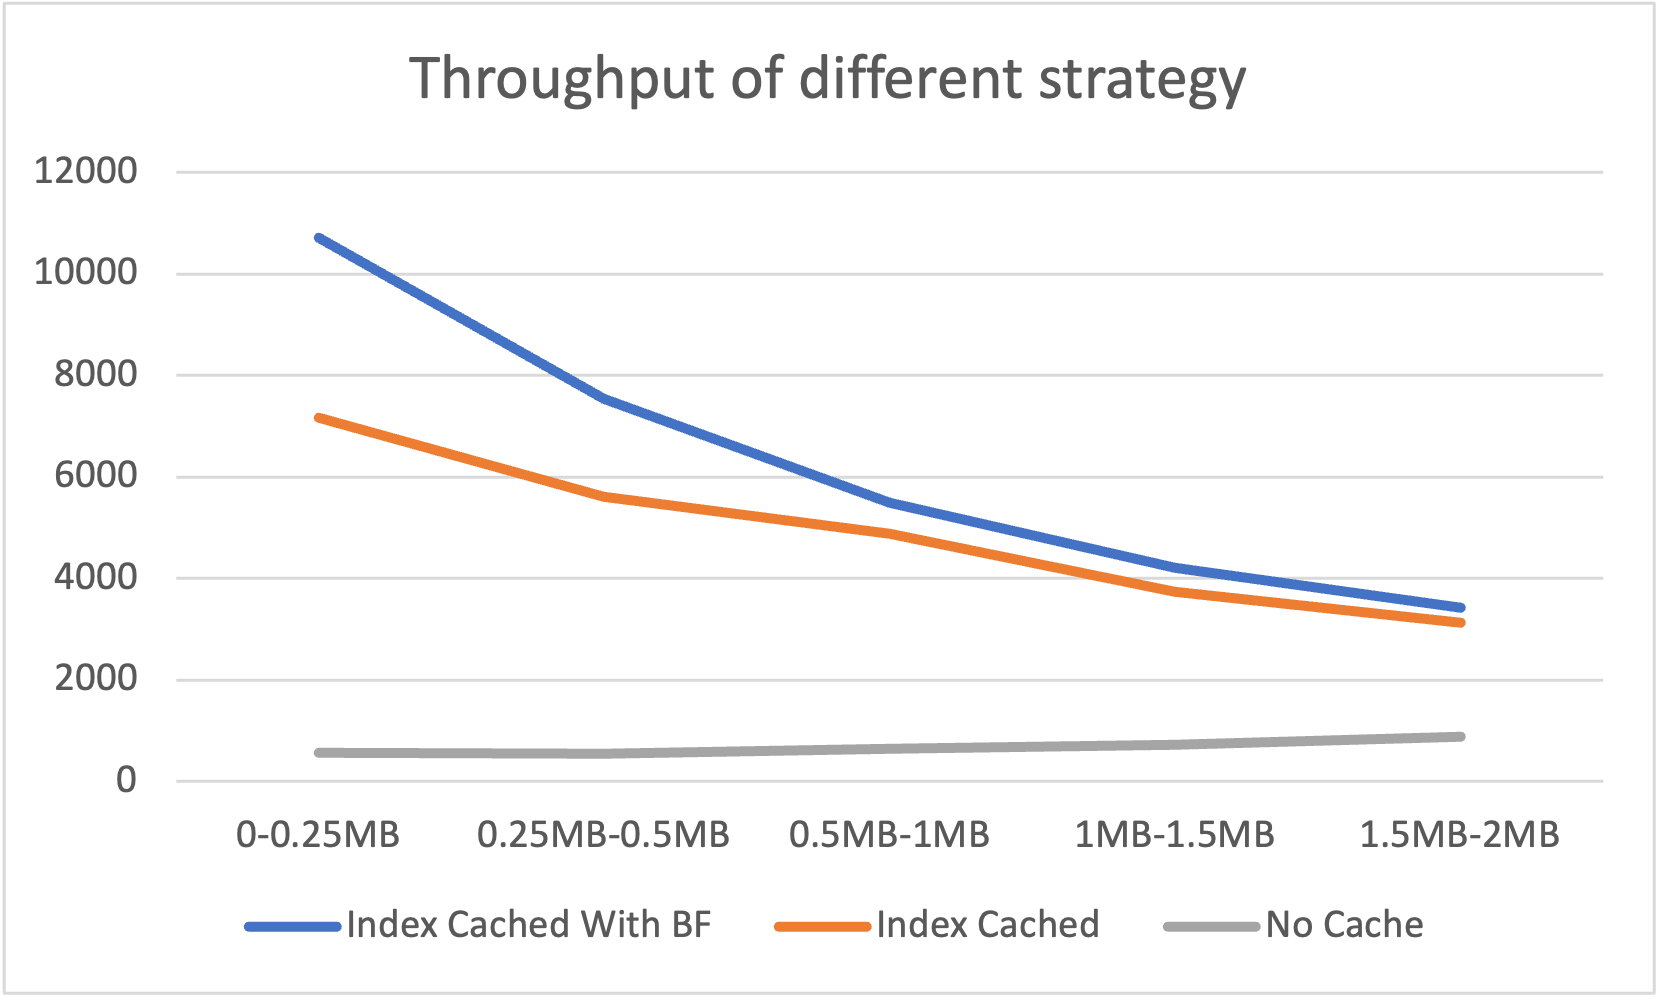
\includegraphics[width=10cm]{Strategy.png}
  \caption{不同策略下的吞吐量}
\end{figure}

\subsubsection{结果分析}
可以看到,三种不同的策略的吞吐量有显著区别。其中有无Bloom Filter在数据量较小时对性能影响较大,原因在于数据量较小时索引量较大,及时是二分查找也需要log(n)的时间,相比Bloom Filter的O(1)复杂度会逊色不少。值得一提的是,在无缓存的策略下,吞吐量反而随着数据量的大小上升而上升,猜测原因在于大数据量下一个SSTable中存的数据反而少,因此在索引过程所花费的时间反而较少。


\subsection{Compaction对PUT操作影响测试}

\subsubsection{测试方法}
计算得出频率为每10次插入就需要1次compaction所需插入的数据大小,随后进行5000次插入(即使compaction大约5000次,数据量在10G左右),其中key的大小随机。测试脚本在compaction.cpp中。

\subsubsection{预期结果}
随时间的增长,因为层数的增加,每次compaction所需时间也越长。

\subsubsection{测试结果}
因篇幅限制,原始数据放在了compaction-test.txt中,以下只放了图:
\begin{figure}[h!]
  \centering
  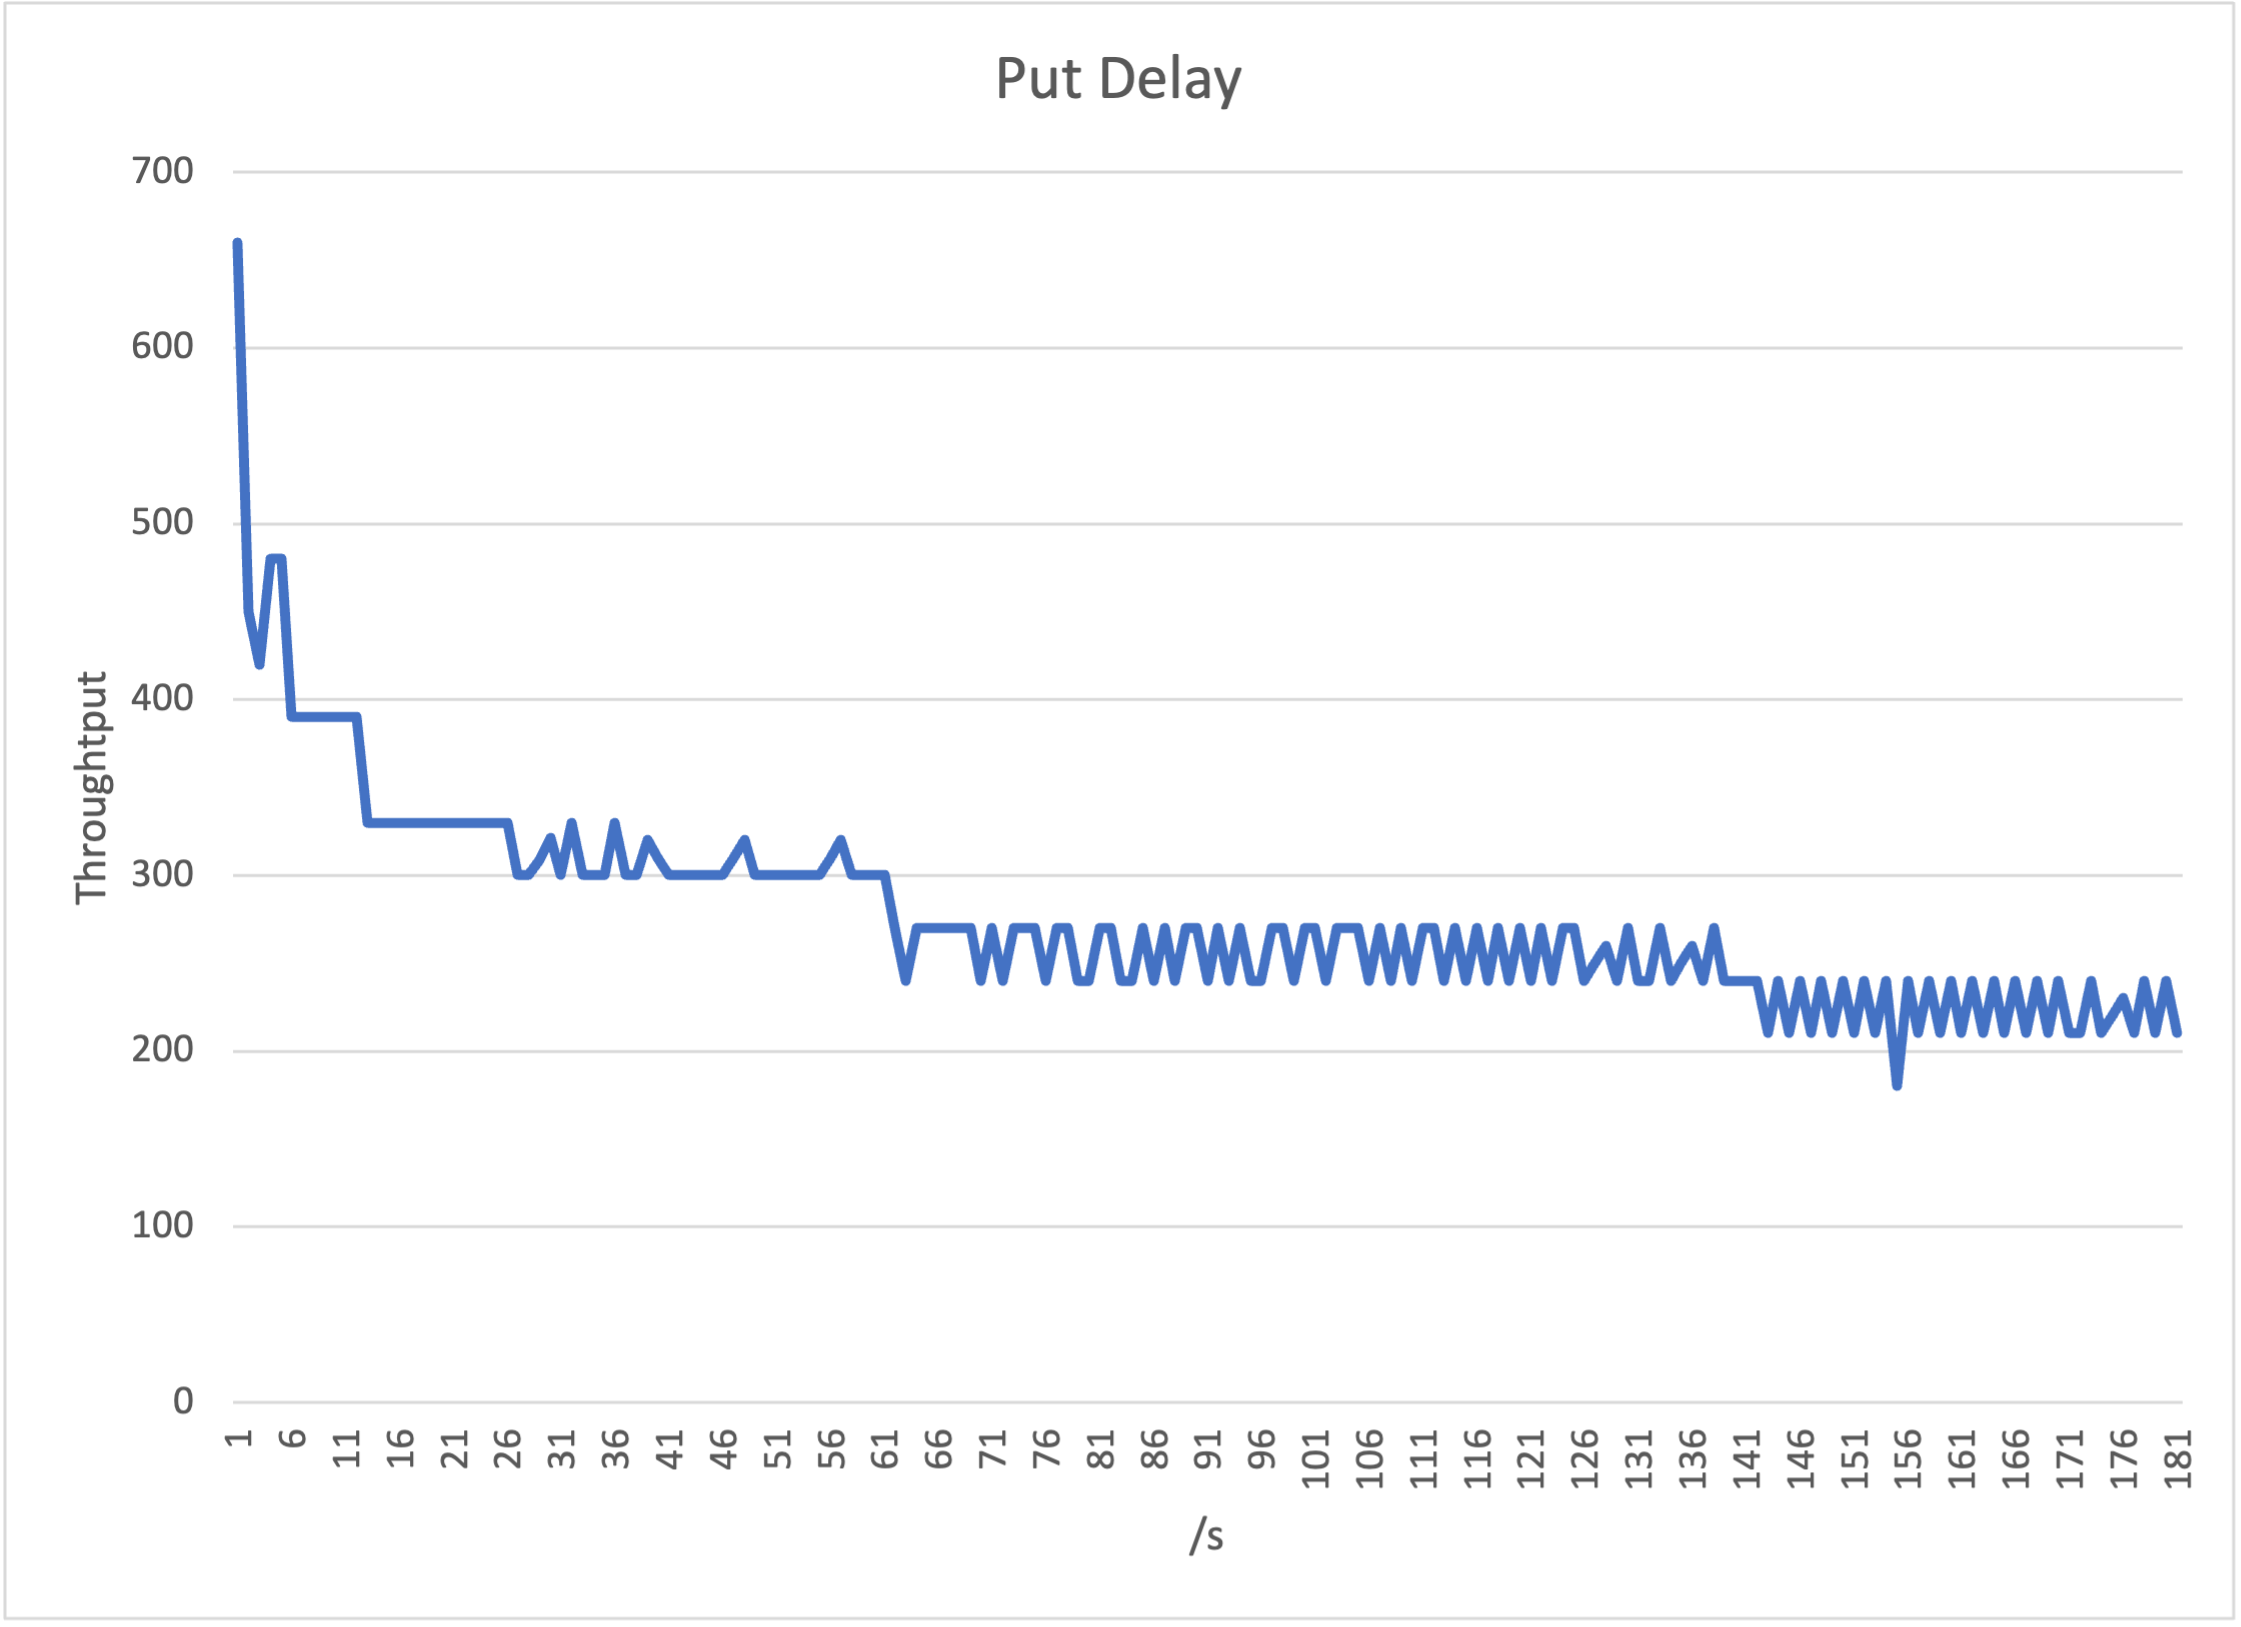
\includegraphics[width=10cm]{Compaction.png}
  \caption{吞吐量随时间变化}
\end{figure}

\subsubsection{结果分析}
可以看到,吞吐量随时间降低。在局部上,呈现锯齿状,猜测每触发一次跨度较大的compaction就会导致该秒内吞吐量骤减;总体来说,呈阶梯状递减趋势,猜测每个阶梯就代表了储存层数的增加。


\subsection{结论}

\subsubsection{收获}
\begin{enumerate}
  \item 完整体验到了实现一个数据结构的流程:写代码,写调试工具,写测试工具。
  \item 使用latex排版报告(非常整齐好看)。
  \item 其余收获见挑战部分。
\end{enumerate}

\subsubsection{建议}
\begin{enumerate}
  \item 建议在测试脚本中增加自动清除本测试产生的数据的选项,需要手动清除很麻烦。
  \item 建议提供校验和查看sst文件的工具,当然不提供也是对综合debug能力提升的一种考验。
  \item 建议SSTable索引区的最后可增加一个空的索引,代表最后一个value结束的offset,可以以很低成本,较大程度地简化读取键值对的逻辑(否则为了读取当前文件的最后一个值,还需要特殊判断是否是最后一个值,计算最后一个值的大小)
\end{enumerate}

\end{document}